\documentclass{article}
\usepackage[utf8]{inputenc}
\usepackage{amsmath}
\usepackage{amssymb}
\usepackage{fancyhdr}
\usepackage{fullpage}
\usepackage{listings}
\usepackage{graphicx}
\pagestyle{fancy}
\lstset{breaklines=true}
\begin{document}

\lhead{M1 Mathématiques \\ Analyse Numérique et Simulation \\ Bastien SAUVAGE et Guillaume ROUMAGE}
\rhead{UPEM \\ Semestre 1 - 2018/2019} 

$$ \textbf{Projet : Simulation~du~système~solaire}$$

\section{Partie Théorique} 
\subsection*{Question 1}
Nous considérons 6 corps que nous noterons $P_i~,~ 1 \leq i\leq 6 $ . \\
Nous devons considérer un corps fixe sur lequel nous fixerons un repère fixe $R_G $. Notons G le centre de masse du soleil et prenons G comme origine de notre repère fixe $R_G $ (repère galiléen).\\
\\
On pose : \\ \\
$ \vec{q_i} = \overrightarrow{GP_i}~,~{q_i} = \parallel\vec{q_i}\parallel~,~\overrightarrow{V_{P_i/R_G}}=\dot{q_i} ~~,~~ 1 \leq i\leq 6 $ \\ \\
$ \overrightarrow{q_{ij}} = \vec{q_j}-\vec{q_i} = \overrightarrow{P_iP_j} = q_{ij}\vec{e_{ij}} ~,~ q_{ij}=\parallel\overrightarrow{q_{ij}}\parallel$
\\ \\
Soit $R_i$ les repères relatifs attaché au centre de chaques corps qui bougent autour du soleil.\\ \\
$  \overrightarrow{V_{P_j/R_i}}=\dot{\overrightarrow{q_{ij}}} ~,~ \overrightarrow{\Gamma_{P_j/R_i}}=\ddot{\overrightarrow{q_{ij}}}$ \\ \\
Appliquons le principe fondamental de la dynamique : \\ Soit $m_i$ la masse du ième corps\\ \\
$ m_i\overrightarrow{\Gamma_{i/R_g}}=\sum\overrightarrow{F_{\to Pi}}=\sum\limits_{j=1,\ i\neq j}^6 \overrightarrow{F_{P_j \to P_i}}=\sum\limits_{j=1,\ i\neq j}^6 Gm_im_j \frac{\overrightarrow{q_{ij}}}{q_{ij}^3} $ \\ \\
Soit avec les notations de l'énoncé \\ \\
$ m_i\ddot{q_i}=\sum\limits_{j=1,\ i\neq j}^6 Gm_im_j \frac{q_j-q_i}{ \|q_j-q_i \|^3} \Longleftrightarrow \ddot{q_i}=\sum\limits_{j=1,\ i\neq j}^6 -Gm_j \frac{q_i-q_j}{ \|q_i-q_j \|^3}$\\  
\subsection*{Question 2}
$p_i$ est la quantité de mouvement, donc $p_i=m_iv_i$.\\ \\
$\frac{1}{2} \sum\limits_{i=1}^6 \frac{1}{m_i}\|p_i\|^2= \sum\limits_{i=1}^6\frac{1}{2}m_i\|v_i\|^2 $       ,~ et ~ $\frac{1}{2}m_i\|v_i\|^2$~ est l'énergie cinétique du $i^{ieme}$\\ \\ corps donc $\frac{1}{2} \sum\limits_{i=1}^6 \frac{1}{m_i}\|p_i\|^2$ est l'énergie cinétique du système.\\ \\
$-\sum\limits_{i=1}^5\sum\limits_{j=i+1}^6G\frac{m_im_j}{\|q_i-q_j\|}$ est l'énergie potentiel du système. \\ \\
\subsection*{Question 3}
Soit $H(p,q)=K(p)+U(q)$ on a \\ \\ $\left \{
   \begin{array}{r c l}
      p'(t)  & = & -\nabla U(q(t)) \\
      q'(t)  & = & \nabla K(p(t)) \\
   \end{array}
   \right. $
   \\ \\
   On pose $\frac{d}{dt}(\|v_i(t)\|^2)=2v_i(t)$ ~ et ~ $\frac{d}{dt}(\frac{1}{\|q_i(t)-q_j(t)\|})=\frac{d}{dt}(\frac{1}{\sqrt{\langle q_i(t)-q_j(t),q_i(t)-q_j(t)\rangle}})$\\ \\
   $=\frac{-\frac{2(q_i(t)-q_j(t))}{2\sqrt{\langle q_i(t)-q_j(t),q_i(t)-q_j(t)\rangle}}}{\|q_i(t)-q_j(t)\|^2} =- \frac{q_i(t)-q_j(t)}{\|q_i(t)-q_j(t)\|^3}$\\ \\
   Donc si on pose, \\ \\ $p_i(t)=\sum\limits_{j=i+1}^6G\frac{m_im_j}{\|q_i(t)-q_j(t)\|} \Longleftrightarrow m_iv_i(t)=\sum\limits_{j=i+1}^6G\frac{m_im_j}{\|q_i(t)-q_j(t)\|} \\\Longleftrightarrow v_i(t)=\sum\limits_{j=i+1}^6G\frac{m_j}{\|q_i(t)-q_j(t)\|} $ \\ En dérivant :  ~$v'_i(t)=\sum\limits_{j=i+1}^6 -Gm_j\frac{q_i(t)-q_j(t)}{\|q_i(t)-q_j(t)\|^3}$ \\ \\
   Ensuite en posant ~ $q_i(t)=\frac{1}{2}\frac{1}{m_i}\|p_i(t)\|^2=\frac{1}{2}m_i\|v_i(t)\|^2$~ \\ \\
   En dérivant on obtient : $q'_i(t)=v_i(t)$. \\ \\
\subsection{Question 4}
$\forall t \in [0,+\infty[ ~~ H(p(t),q(t))=H(p(0),q(0))$\\ \\
Il y a conservation du Hamiltonnien.\\
\\
\section{Résolution Numérique}
\subsection*{Données}
Les données sont stockées dans des tableaux (\textit{array}).
\begin{itemize}
\item Les noms des planètes sont stockés dans un tableau de dimensions 6. Leurs couleurs par lesquelles elles sont représentées sur la simulation est également stocké.
\item Les masses des planètes sont stockées dans un tableau de dimensions 6.
\item Les positions initiales sont stockées dans un tableau de dimensions 6x3. Dans chaque cases se trouve un tableau de dimension 3 dans lequel est stocké la position initiale en x, en y et en z.
\item Les vitesses initiales sont stockées dans un tableau de dimensions 6x3. Dans chaque cases se trouve un tableau de dimension 3 dans lequel est stocké la position initiale en x, en y et en z.
\end{itemize}
\subsection*{Question 5}
Afin d'avoir les distances, en unités astronomiques entre le Soleil et les 5 autres planètes, on execute le code suivant.
\begin{lstlisting}
def distance_soleil_ini():
    for i in range(1, nb_planets):
        print("La distance au 1er septembre 2012 a 00h00 entre " + planet[i] + " et le Soleil est : " + str(linalg.norm(pos_ini[i])) + " ua.")
\end{lstlisting}
Le résultat affiché est :
\begin{lstlisting}
La distance au 1er septembre 2012 a 00h00 entre Jupiter et le Soleil est : 5.02722412544 ua.
La distance au 1er septembre 2012 a 00h00 entre Saturne et le Soleil est : 9.75997406864 ua.
La distance au 1er septembre 2012 a 00h00 entre Uranus et le Soleil est : 20.0644174946 ua.
La distance au 1er septembre 2012 a 00h00 entre Neptune et le Soleil est : 29.9945592007 ua.
La distance au 1er septembre 2012 a 00h00 entre Pluton et le Soleil est : 32.2906462191 ua.
\end{lstlisting}
Dans la suite, les différents corps seront numérotés de 1 à 6. $q_i(t)$ et $v_i(t)$ sont la position et la vitesse du corps $i$ au temps $t$.
\subsection*{Question 6}
On reprends les notations usuelles du cours.\\
Les formules de la méthodes d'Euler appliquées au système donnent, pour $1 \leq i \leq 6$ et $t \in [0;T]$ :
$$\left\{
\begin{array}{l l}
q_i'(t) = q_i(t) + h.v_i(t) \\
v_i'(t) = v_i(t) + h.\sum\limits_{\underset{i \neq j}{1 \leq j \leq 6}} -Gm_j\frac{q_i(t)-q_j(t)}{||q_i(t)-q_j(t)||^3}
\end{array}
\right.$$
\subsection*{Question 7}
\begin{lstlisting}[language=Python]
def calc_energy(pos, vit):
    a = 0
    b = 0
    for i in range(nb_planets):
        a = a + masse[i] * linalg.norm(vit[i])**2
    for i in range(5):
        for j in range(i+1, 6):
            b = b + g * (masse[i] * masse[j])/(linalg.norm(pos[i] - pos[j]))
    return 1/2 * a - b

def calc_vit(i, pos):
    res = array([0.,0.,0.])
    for j in range (0, nb_planets):
        if i != j:
            res = res - g * masse[j] * (pos[i] - pos[j])/(linalg.norm(pos[i] - pos[j])**3)
    return res
    
def solaire_euler(dt, N):
    [...]
    for i in range(1, length):
        pos_next = pos_old + dt * vit_old
        vit_next = vit_old + dt * array([calc_vit(0,pos_old),calc_vit(1,pos_old),calc_vit(2,pos_old),calc_vit(3,pos_old),calc_vit(4,pos_old),calc_vit(5,pos_old)])
        energy[i] = calc_energy(pos_next, vit_next)
        pos[i] = pos_next
        pos_old = pos_next
        vit_old = vit_next
	[...]
\end{lstlisting}
\subsection*{Question 8}
On reprends les notations usuelles du cours.\\
Les formules de la méthodes de Störmer-Verlet appliquées au système donnent, pour $1 \leq i \leq 6$ et $t \in [0;T]$ :
$$\left\{
\begin{array}{l l}
q_{i,1}(t) = q_i(t) + \frac{h}{2}.v_i(t) \\
v_i'(t) = v_i(t) + h.\sum\limits_{\underset{i \neq j}{1 \leq j \leq 6}} -Gm_j\frac{q_i(t)-q_j(t)}{||q_i(t)-q_j(t)||^3} \\
q_i'(t) = q_{i,1}(t) + \frac{h}{2}.v_i'(t)
\end{array}
\right.$$
\subsection*{Question 9}
\begin{lstlisting}[language=Python]
def solaire_stormer_verlet(dt, N):
    [...]
    for i in range(1, length):
        pos_inter = pos_old + dt/2 * vit_old
        vit_next = vit_old + dt * array([calc_vit(0,pos_old),calc_vit(1,pos_old),calc_vit(2,pos_old),calc_vit(3,pos_old),calc_vit(4,pos_old),calc_vit(5,pos_old)])
        pos_next = pos_inter + dt/2 * vit_next
        energy[i] = calc_energy(pos_next, vit_next)
        pos[i] = pos_next
        pos_old = pos_next
        vit_old = vit_next
    [...]
\end{lstlisting}
\newpage
\subsection*{Question 10}
\begin{figure}[!h]
\begin{center}
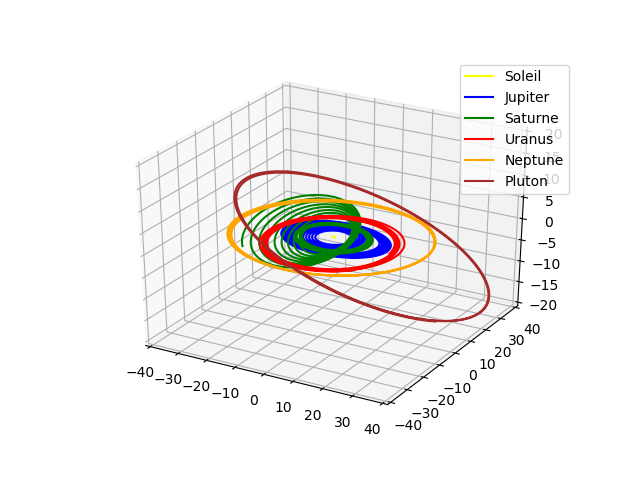
\includegraphics[scale=0.65]{Simulation_euler.png}
\caption{Simulation du système solaire avec la méthode d'euler explicite sur 200 000 jours avec un pas de 10 jours}
\end{center}
\end{figure}
\begin{figure}[!h]
\begin{center}
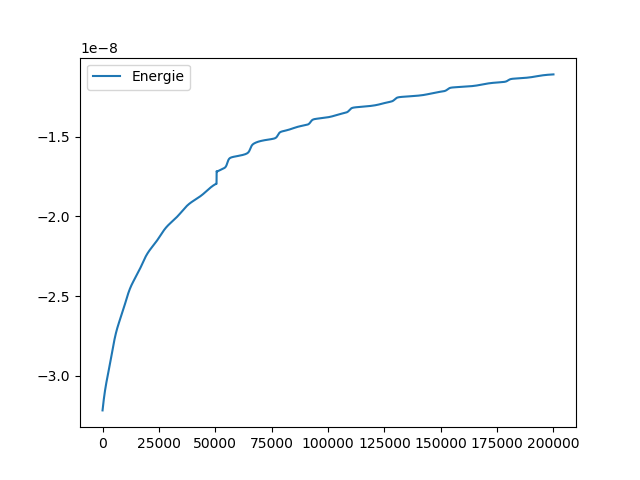
\includegraphics[scale=0.65]{Hamiltonien_euler.png}
\caption{Evolution du hamiltonien lors de la simulation du système solaire avec la méthode d'euler explicite sur 200 000 jours avec un pas de 10 jours}
\end{center}
\end{figure}
\newpage
\begin{figure}[!h]
\begin{center}
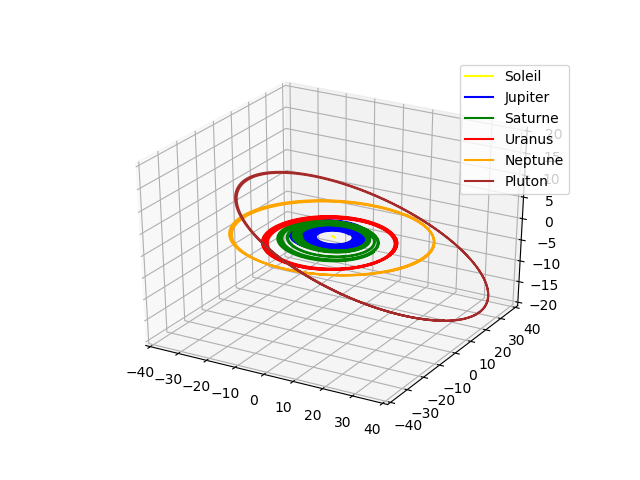
\includegraphics[scale=0.7]{Simulation_stormer_verlet.png}
\caption{Simulation du système solaire avec la méthode de Störmer-Verlet sur 200 000 jours avec un pas de 10 jours}
\end{center}
\end{figure}
\begin{figure}[!h]
\begin{center}
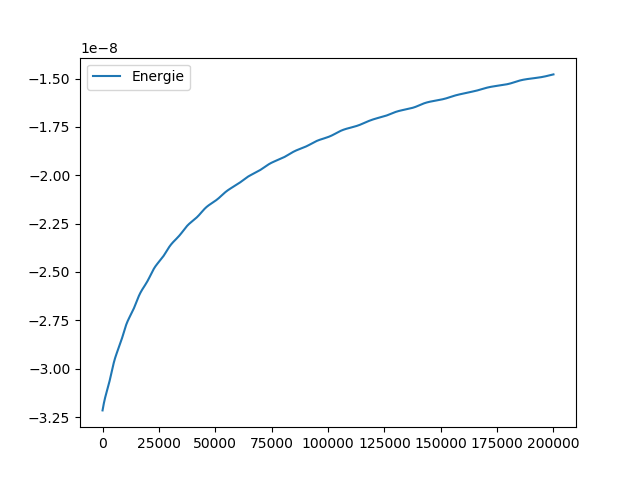
\includegraphics[scale=0.7]{Hamiltonien_stormer_verlet.png}
\caption{Evolution du hamiltonien lors de la simulation du système solaire avec la méthode de Störmer-Verlet sur 200 000 jours avec un pas de 10 jours}
\end{center}
\end{figure}
\newpage
\begin{figure}[!h]
\begin{center}
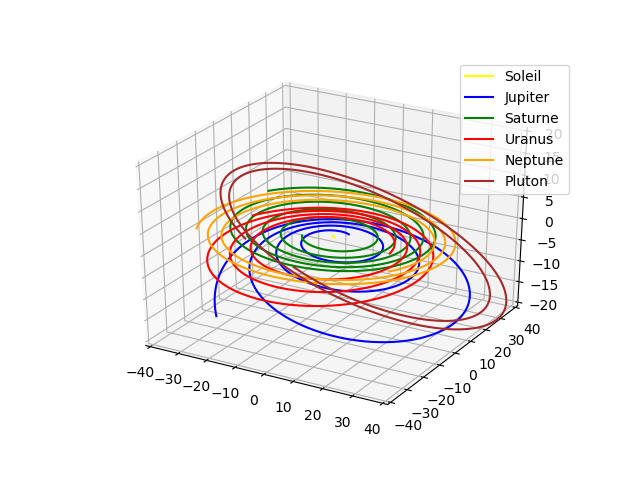
\includegraphics[scale=0.7]{Simulation_stormer_verlet_200.png}
\caption{Simulation du système solaire avec la méthode de Störmer-Verlet sur 200 000 jours avec un pas de 200 jours}
\end{center}
\end{figure}
\begin{figure}[!h]
\begin{center}
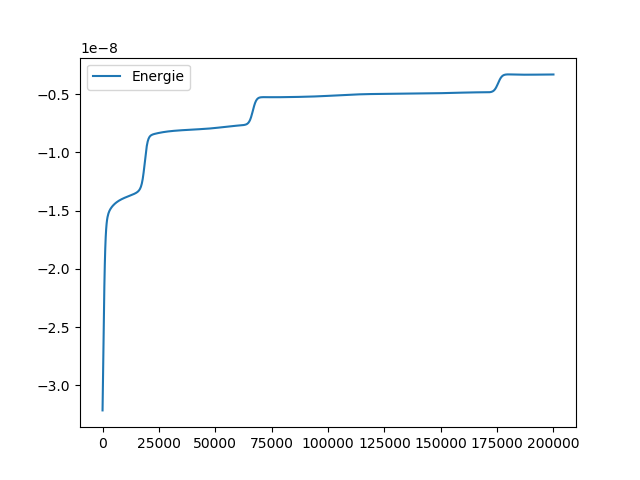
\includegraphics[scale=0.7]{Hamiltonien_stormer_verlet_200.png}
\caption{Evolution du hamiltonien lors de la simulation du système solaire avec la méthode de Störmer-Verlet sur 200 000 jours avec un pas de 200 jours}
\end{center}
\end{figure}
\newpage
\noindent
Pour un même pas de temps et une même période d'étude, on remarque que la méthode de Störmer-Verlet donne des trajectoires de planètes plus préçises que celles d'Euler explicite. Le calcul du hamiltonien est également plus préçis, avec moins de perturbations.\\
Lorsque l'on utilise la méthode de Störmer-Verlet sur 200 000 jours avec un pas de 200 jours, les calculs sont plus rapides mais les trajectoires sont très perturbées. Le hamiltonien est également moins bien calculé que dans les deux simulations précédentes. Un pas de 200 jours avec la méthode de Störmer-Verlet est donc trop grand dans cette simulation.\\
\\
Dans tout les cas, le hamiltonien n'est pas conservé alors qu'il devrait rester constant. Cela est dû au fait que les méthodes utilisées ne sont pas des méthodes symplectiques.
\subsection*{Question 11}
Pour calculer la révolution de Neptune et de Pluton, utilise l'algorithme suivante.
\begin{enumerate}
\item On calcule les positions successives des planètes aux différents pas de temps, sur tout l'intervalle étudié, comme lors d'une simulation (on utilise la méthode de Störmer-Verlet).
\item A chaque pas de temps, on calcule la distance entre la position courante de la planète et sa position initiale. Celle-ci est stockée au fur et à mesure.
\item A la fin de la simulation, on recherche le minimum de ces distances. Cette distance minimale correspondond à un certains temps $t_n$. Pour trouver la période de révolution, il suffit donc de multiplier $t_n$ par le $dt$ utilisé.
\end{enumerate}
Notons que la recherche du minimum commence à la 100-ème case du tableau de stockage pour s'assurer que la planète a fait au moins une révolution.\\
En effet, si la recherche commence dès la case 0, la distance minimale qui sera calculée pourrait être la distance entre la position initiale et une position situé à quelques pas de temps après le temps initiale, auquel cas la planète n'aura pas encore fait de révolution. Le calcul serait donc faussé.
\begin{lstlisting}[language=Python]
def indice_min(tab):
    min = tab[100]
    ind_min = 100
    for i in range(101, len(tab)):
        if tab[i] < min:
            ind_min = i
            min = tab[i]
    return ind_min
    
def revolution(dt, N):
    [...]
    for i in range(1, length):
        pos_inter = pos_old + dt/2 * vit_old
        vit_next = vit_old + dt * array([calc_vit(0,pos_old),calc_vit(1,pos_old),calc_vit(2,pos_old),calc_vit(3,pos_old),calc_vit(4,pos_old),calc_vit(5,pos_old)])
        pos_next = pos_inter + dt/2 * vit_next
        pos[i] = pos_next
        pos_old = pos_next
        vit_old = vit_next
        distance_nep[i] = linalg.norm(pos_next[4] - pos_ini[4])
        distance_plu[i] = linalg.norm(pos_next[5] - pos_ini[5])
    print("La periode de revolution de Neptune est de " + str(indice_min(distance_nep) * dt) + " jours.")
    print("La periode de revolution de Pluton est de " + str(indice_min(distance_plu) * dt) + " jours.")
\end{lstlisting}
Les résultats sont les suivants :
\begin{lstlisting}[language=Python]
La periode de revolution de Neptune est de 60510 jours.
La periode de revolution de Pluton est de 90940 jours.
\end{lstlisting}
\subsection*{Question 12}
La fonction d'animation utilisée est la suivante.
\begin{lstlisting}[language=Python]
def solaire_anime(dt, N):
    [...]
    for n in range(1, length):
        pos_inter = pos_old + dt/2 * vit_old
        vit_next = vit_old + dt * array([calc_vit(0,pos_old),calc_vit(1,pos_old),calc_vit(2,pos_old),calc_vit(3,pos_old),calc_vit(4,pos_old),calc_vit(5,pos_old)])
        pos_next = pos_inter + dt/2 * vit_next
        
        x[n] = array([pos_next[0][0],pos_next[1][0],pos_next[2][0],pos_next[3][0],pos_next[4][0],pos_next[5][0]])
        y[n] = array([pos_next[0][1],pos_next[1][1],pos_next[2][1],pos_next[3][1],pos_next[4][1],pos_next[5][1]])
        z[n] = array([pos_next[0][2],pos_next[1][2],pos_next[2][2],pos_next[3][2],pos_next[4][2],pos_next[5][2]])
        
        pos_old = pos_next
        vit_old = vit_next
        
        for pt,line,i in zip(pts,lines,range(6)):
            line.set_data(x[:n,i],y[:n,i])
            line.set_3d_properties(z[:n,i])
            pt.set_data(x[n,i],y[n,i])
            pt.set_3d_properties(z[n,i])
            
        plt.pause(0.00001)
    [...]
\end{lstlisting}
\end{document}